\setchoices{label=(\Alph*)}

\begin{question}[index=1]
设 $g(x)$ 在 $x=0$ 的某邻域内连续，$f(x)$ 具有一阶连续导数，且满足
\[
\lim_{x\to0}\frac{g(x)}x=-3,\qquad f'(x)=\ln(1+x^2)-x\int_0^1 g(xt)\dd t\text{，}
\]
则
\begin{choices}[columns=2]
\item $x=0$ 是 $f(x)$ 的极大值点．
\item $x=0$ 是 $f(x)$ 的极小值点．
\item $(0,f(0))$ 是曲线 $y=f(x)$ 的拐点．
\item 以上说法均不正确．
\end{choices}
\end{question}
\QuestionBreak

\begin{question}[index=2]
设 $\displaystyle f(x,y)=\begin{cases}
x\cos\dfrac1y+y\cos\dfrac1x,&xy\ne0,\\[3pt]
0,&xy=0,
\end{cases}$
以下三个结论：\par
① $\displaystyle\lim_{x\to0}\lim_{y\to0} f(x,y)$ 存在；\par
② $\displaystyle\lim_{y\to0}\lim_{x\to0} f(x,y)$ 不存在；\par
③ $\displaystyle\lim_{(x,y)\to(0,0)} f(x,y)=0$．\par
正确结论的个数为
\begin{choices}[columns=4]
\item $0$．
\item $1$．
\item $2$．
\item $3$．
\end{choices}
\end{question}
\QuestionBreak

\begin{question}[index=3]
设函数 $f(x)$ 在区间 $[a,b]$ 上可积，则以下四个结论：\par
① 当 $\displaystyle\int_a^b f^2(x)\dd x=0$ 时，在 $[a,b]$ 上恒有 $f(x)=0$；\par
② 存在 $\xi\in[a,b]$，使得 $\displaystyle\int_a^b f(x)\dd x=f(\xi)(b-a)$；\par
③ 当 $x\in[a,b]$ 时，有 $\displaystyle\frac{\mathrm d}{\mathrm dx}\left[\int_a^x f(t)\dd t\right]=f(x)$；\par
④ 当 $x\in[a,b]$ 时，有 $\displaystyle\frac{\mathrm d}{\mathrm dx}
\left[\int_a^x f(t)\dd t+\int_x^b f(t)\dd t\right]=0$．\par
正确结论的个数为
\begin{choices}[columns=4]
\item $4$．
\item $3$．
\item $2$．
\item $1$．
\end{choices}
\end{question}
\QuestionBreak

\begin{question}[index=4]
设面密度为 $1$ 的均匀薄板是由 $y=x^2$ 及 $y=1$ 所围成的有界区域，记为 $D$，
则该薄板对直线 $l:y=-1$ 的转动惯量为
\begin{choices}[columns=2,label-pos=left]
\item $\displaystyle\iint_D(y+1)^2\dd x\dd y$．
\item $\displaystyle\iint_D(y-1)^2\dd x\dd y$．
\item $\displaystyle\iint_D(x-1)^2\dd x\dd y$．
\item $\displaystyle\iint_D(x+1)^2\dd x\dd y$．
\end{choices}
\end{question}
\QuestionBreak

\begin{question}[index=5]
已知向量组
\[
\symbfit\beta_1=\begin{pmatrix}0\\1\\-1\end{pmatrix},\quad
\symbfit\beta_2=\begin{pmatrix}a\\2\\1\end{pmatrix},\quad
\symbfit\beta_3=\begin{pmatrix}b\\1\\0\end{pmatrix}
\]
与向量组
\[
\symbfit\alpha_1=\begin{pmatrix}1\\2\\-3\end{pmatrix},\quad
\symbfit\alpha_2=\begin{pmatrix}3\\0\\1\end{pmatrix},\quad
\symbfit\alpha_3=\begin{pmatrix}9\\6\\-7\end{pmatrix}
\]
具有相同的秩，且 $\symbfit\beta_3$ 可由 $\symbfit\alpha_1,\symbfit\alpha_2,\symbfit\alpha_3$
线性表示，则 $(a,b)=$
\begin{choices}[columns=4]
\item $(5,15)$．
\item $(15,5)$．
\item $(6,18)$．
\item $(18,6)$．
\end{choices}
\end{question}
\QuestionBreak

\begin{question}[index=6]
已知 $f(x_1,x_2,x_3)=\symbfit x^{\mathrm T}\symbfit A\symbfit x$
经正交变换 $\symbfit x=\symbfit Q\symbfit y$ 化为
$g(y_1,y_2,y_3)=y_1^2+2y_2^2+ay_3^2\ (a\ne0)$，且
\[
\symbfit Q^{-1}\symbfit A^*\symbfit Q=\begin{pmatrix}1&0&0\\0&\dfrac12&0\\0&0&\dfrac1a\end{pmatrix},
\]
其中 $\symbfit A^*$ 是 $\symbfit A$ 的伴随矩阵，则对任意 $\symbfit x\ne\symbf0$，有
\begin{choices}[columns=2]
\item $f(x_1,x_2,x_3)>0$．
\item $f(x_1,x_2,x_3)=0$．
\item $f(x_1,x_2,x_3)<0$．
\item $f(x_1,x_2,x_3)\le0$．
\end{choices}
\end{question}
\QuestionBreak

\begin{question}[index=7]
线性方程组 $\begin{cases}
x_1+x_2+ax_3=4,\\
x_1-x_2+2x_3=-4,\\
-x_1+ax_2+x_3=a^2
\end{cases}$ 所代表的三个平面不可能的位置关系为
\begin{choices}[columns=2,label-pos=left]
\item 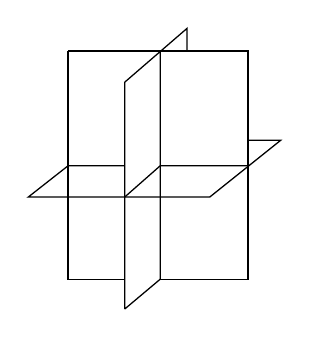
\begin{tikzpicture}[x=.018cm,y=-.018cm,baseline=(current bounding box.center),line width=.46pt]
  \draw (28,20)--(155,20)--(155,181)--(93,181) (68,181)--(28,181)--(28,122)--(28,20);
  \draw (68,202)--(93,181)--(93,20) (68,202)--(68,42)--(112,4)--(112,20);
  \draw (28,101)--(68,101) (155,83)--(178,83)--(128,123)--(0,123)--(28,101);
  \draw (68,123)--(93,101)--(155,101);
\end{tikzpicture}
\item 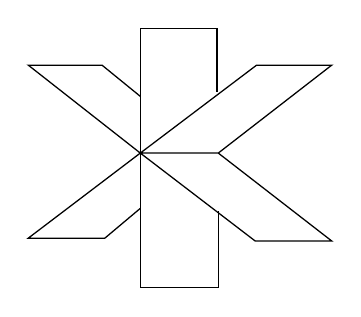
\begin{tikzpicture}[x=.018cm,y=-.018cm,baseline=(current bounding box.center),line width=.46pt]
  \draw (79,88)--(79,0)--(133,0)--(133,45);
  \draw (79,88)--(0,26)--(52,26)--(79,48);
  \draw (79,88)--(0,148)--(54,148)--(79,127);
  \draw (79,88)--(79,183)--(134,183)--(134,129);
  \draw (79,88)--(161,26)--(214,26)--(134,88)--(214,150)--(160,150)--(79,88)--(134,88);
\end{tikzpicture}
\item 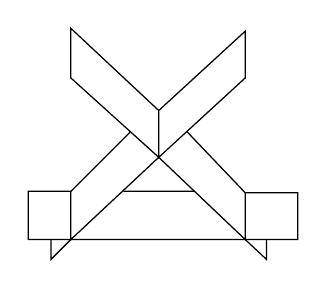
\begin{tikzpicture}[x=.018cm,y=-.018cm,baseline=(current bounding box.center),line width=.46pt]
  \draw (92,91)--(30,35)--(30,0)--(92,58)--(153,2)--(153,35)--(92,91)--(92,58);
  \draw (72,73)--(30,115)--(0,115)--(0,149)--(190,149)--(190,116)--(153,116)--(112,73);
  \draw (30,115)--(30,149)--(92,91)--(153,149)--(153,116);
  \draw (67,115)--(117,115) (16,149)--(16,163)--(30,149) (153,149)--(168,163)--(168,149);
\end{tikzpicture}
\item 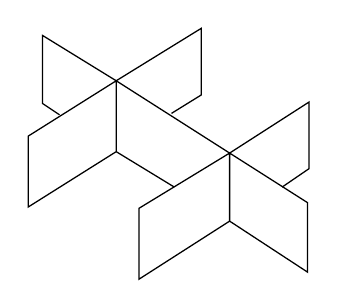
\begin{tikzpicture}[x=.018cm,y=-.018cm,baseline=(current bounding box.center),line width=.46pt]
  \draw (62,37)--(10,5)--(10,53)--(22,61);
  \draw (62,37)--(122,0)--(122,47)--(101,60);
  \draw (62,37)--(0,76)--(0,126)--(62,87)--(62,37)--(142,88);
  \draw (62,87)--(103,112);
  \draw (142,88)--(198,52)--(198,99)--(179,112);
  \draw (142,88)--(78,127)--(78,177)--(142,136)--(142,88)--(197,123)--(197,172)--(142,136);
\end{tikzpicture}
\end{choices}
\end{question}
\QuestionBreak

\begin{question}[index=8]
假设 $\{X_n\}\ (n\ge1)$ 为独立同分布的连续型随机变量序列，其概率密度为 $f(x)$，
分布函数 $F(x)$ 是 $x$ 的严格单调函数，则
$\displaystyle\lim_{n\to\infty}P\left\{\frac1n\sum_{i=1}^n F(X_i)\le\frac12\right\}=$
\begin{choices}[columns=4,label-pos=left]
\item $\dfrac13$．
\item $\dfrac12$．
\item $\dfrac23$．
\item $1$．
\end{choices}
\end{question}
\QuestionBreak

\begin{question}[index=9]
设连续型随机变量 $X$ 的分布函数为 $F(x)$，$EX=\mu$，$DX=\sigma^2\ (\sigma>0)$，
若随机变量 $Y$ 的分布函数为 $\displaystyle G(y)=F\left(\frac{y-\mu}{\sigma}\right)$，
则 $EY$ 和 $DY$ 分别为
\begin{choices}[columns=4,label-pos=left]
\item $\dfrac{\mu}{\sigma+1},\sigma^4$．
\item $\mu(\sigma+1),\sigma^4$．
\item $\dfrac{\mu}{\sigma+1},\sigma^2$．
\item $\mu(\sigma+1),\sigma^2$．
\end{choices}
\end{question}
\QuestionBreak

\begin{question}[index=10]
已知总体 $X$ 的概率密度为
\[
f(x)=\frac12\mathrm e^{-|x-\theta|},\quad -\infty<x<+\infty,
\]
$x_1\le x_2\le\cdots\le x_{10}$ 是来自该总体的简单随机样本的观察值，
则 $\theta$ 的最大似然估计值为
\begin{choices}[columns=4,label-pos=left]
\item $\dfrac{x_5}2$．
\item $\dfrac{x_6}2$．
\item $\dfrac{x_6-x_5}2$．
\item $\dfrac{x_5+x_6}2$．
\end{choices}
\end{question}
